\section{Cooperation Spectrum}
To learn how cooperative behaviors may influence success ratio in a particular task, the decision was made to first observe the evolution in case where agents work against one another, competing for a higher score. Only then, comparing the results with those of a cooperative case, conclusions regarding cooperation influence may be drawn.
The scenarios were tested in parallel with each change, were it to complicate the problem or put emphasis on certain components of the solutions.

The two scenarios shall be described in their dedicated sections below, focusing on key contrast points. Following, however, are the elements common to both cases.

Evaluation process of candidate solutions was made in the same environment, with identical starting points and resource markers' locations. In both scenarios, trees produced by Genetic Programming are accompanied by a unchanging, user-defined tree in the simulations. This reference agent uses one type of Action, \textit{goToFlag(flagNumber)}, visiting each resource marker in turn, capturing them from first to last, never changing path between simulations. Figure \ref{fig:x referenceagentdiagram} presents the Behavior Tree schematic of the reference agent. Existence of such tree could fill the function of both a pressuring component (reflected in the fitness function in the appropriate cases) and essentialy a time-gate, as gathering all markers would end the simulation. Furthermore, algorithms in both cases had access to identical Behavior Tree Components to build the trees from, thus ensuring equal sophistication of solutions in each scenario.

\begin{figure}[h]
    \centering
    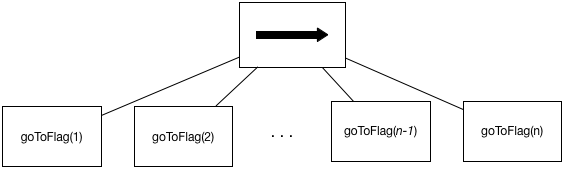
\includegraphics[scale=0.4]{referenceagentdiagram}
    \caption{A scematic of reference agent used in simulations.}
    \label{fig:x referenceagentdiagram}
\end{figure}
Finally, the three components that partook in the specimen grading were as follows:
\begin{itemize}
    \item \textbf{Number of markers gathered} - a number of resource markers gathered.
    \item \textbf{Time to completion} - how much time did it take to finish the simulation (i.e. how much time has elapsed untill all the markers were claimed).
    \item \textbf{Size of a Tree} - how many nodes were in the tree.
\end{itemize}
% mention the task? the role of each component in producing optimal tree? define desirable solution?
% also, is it worth mentioning that the agents wouldn't know if the flag is claimed before getting there?
\section{Competitive Scenario Specification}
\subsection{Synopsis}
Competitive case assumed the optimal solution to the problem is maximizing the agent's personal gain. The markers gathered were counted separably for each agent, thus turning the task into a race - evolutionary agent was forced to get to as many markers as possible before the reference agent would claim them for himself.

After initial testing, the scenario was modified to feature 7 resource markers (instead of initial 5) and modified spawn points of agents -  readjusted to move evolutionary agent further back from the first marker. While increasing the number of markers served as an attempt to complicate the problem, moving evolutionary agent further from the first flag was done in the interest of being able to reproduce the results: since both agents were in the equal distance of the first flag and moved with the same speed, the matter of which one would claim the first flag was comparable to a coin-toss. Figure \ref{fig:x scenario1topdown} presents the final view of the competitive scenario map.

\begin{figure}[h]
    \centering
    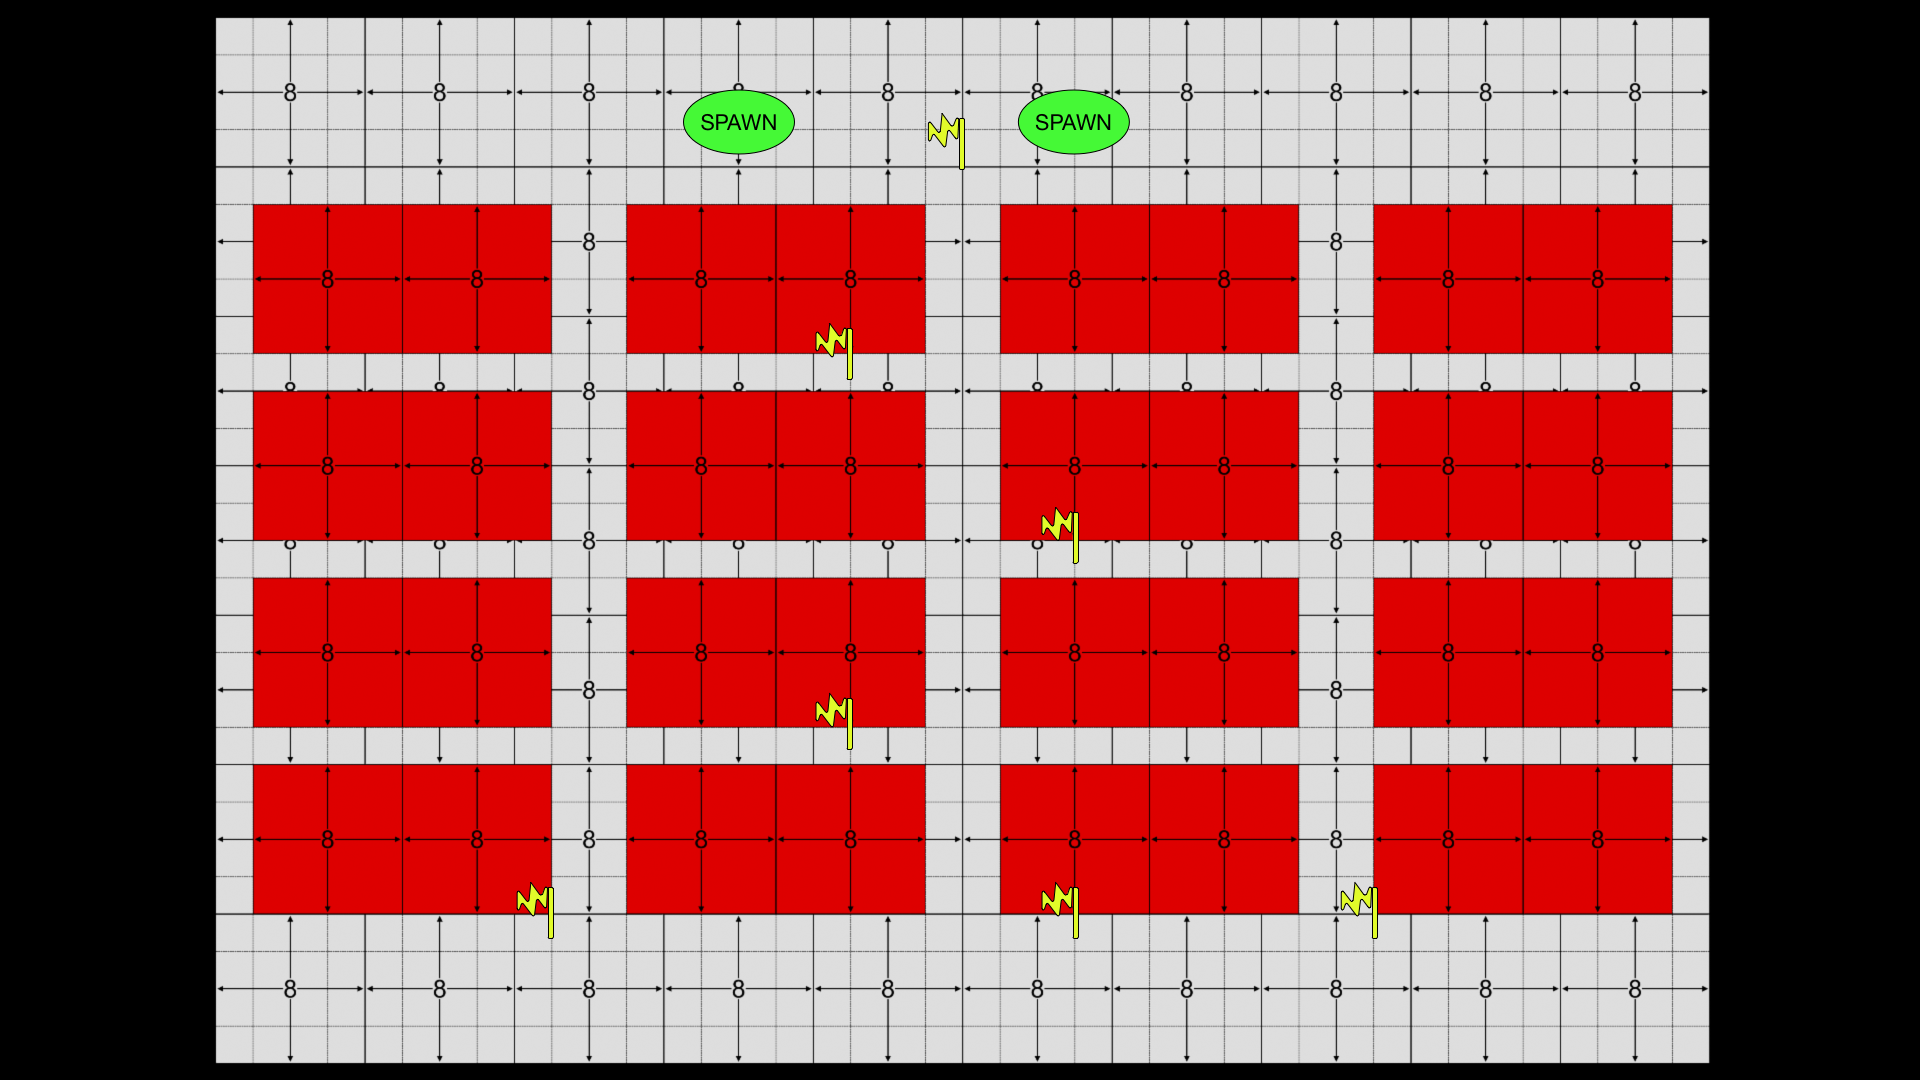
\includegraphics[scale=0.2]{scenario1topdown}
    \caption{Finished map of the competitive scenario environment}
    \label{fig:x scenario1topdown}
\end{figure}

\subsection{Fitness Function} % should it include a plot of a fitness function?
The competitive scenario is effectively a zero-sum game. Considering that, the initial fitness value of the $i-th$ specimen in the population was a sum of $n$ markers gathered by an agent controlled by a tested tree, multiplied by a resource point constant $C_1$. This, however, wasn't feasible as a long-term solution. To introduce differentiability between the specimen scoring the same amounts of markers, a  factor of time in miliseconds multiplied by constant $C_2$ was then subtracted from the sum. Additionally, to coerce the algorithm into preferring smaller trees, a tree size factor with weight $C_3$ was further subtracted from this value. The finished formula for fitness function is presented on Equation \ref{eq:x scenario1fitness}.
\begin{equation}
    \label{eq:x scenario1fitness}
f(i) = C_1 * n - (\frac{t}{C_2} + \frac{s}{C_3})
\end{equation}
\subsection{Success Criterion}
With the goal of maximizing personal gain, which is the case with the considered scenario, desirable trees are those that claim every possible marker. However, since evolutionary agent's spawn position put it at the disadvantage (making it impossible to gather the first flag), only solutions with $n-1$ flags gathered out of $n$ possbile would be considered ``successful''. The true goal of a ideal solution was then to create a big enough difference in time taken to visit the markers, allowing it to reach and claim the last one.
\section{Cooperative Scenario Specification}
\subsection{Synopsis}
Cooperative scenario, in contrast to the ``selfishly'' motivated competitive one, takes a broader perspective. Instead of competing, agents were expected to work with each other towards claiming all 5 markers. However in time, the layout of the scenario was modified to maintain uniformity between the two cases' layout - that included both increasing the number of flags to 7 and modifying the agents' spawn positions - for comparison reasons.
\subsection{Fitness Function}
Due to competitive aspect being gone, a perspective on performance shifted substiantially. The number of markers claimed by an agent became an impractical characteristic, with the time factor providing a much more considerable view on specimen performance. However, the decision was made to include the \textit{total number of markers} in the fitness function, serving as a constant, to ensure that the results from both scenarios are of the same order of magnitude. Aforementioned time and tree size components remained in untouched form, all the more critical in case at hand. Equation \ref{eq:x scenario2fitness} presents the fitness function used in evaluating specimen in cooperative scenariio.
\begin{equation}
    \label{eq:x scenario2fitness}
f(i) = C_1 * (n + m) - (\frac{t}{C_2} + \frac{s}{C_3})
\end{equation} % legend?

\subsection{Success Criterion}
In the cooperative case, the underlaying goal is to divide the markers between two agents in the most efficient way. To effectively operate, the desired outcome is achieving completion time shorter than the time it takes for the reference agent to complete his route. In other words, a successful solution wille be able to successfuly adapt itself to a potential parter's route and act accordingly. % reword to make it clearer?

\section{Genetic Programming Parameters in Experiments}
After observing the results from a number of initial test runs as well as using \textit{grid-search} algorithm to help determine \textit{crossover rate}, \textit{mutation rate} and \textit{population size} parameters, the parameters used in the experiments are presented in table \ref{table:x selectedparameters}

\begin{table} [h]
    \centering
    \begin{tabular} {c c}
        \hline \hline
        Parameter Name & Parameter Value \\
        \hline
        Maximum Number of Generations & 100 \\
        Population Size & 200 \\
        Crossover Rate & 25\% \\
        Micromutation Rate & 15\% \\
        Macromutation Rate & 2\% \\
        Tournament Selection Tourney Size & 10 \\
        Starting Generation Minimum Tree Size & 20 \\
        Starting Generation Maximum Tree Size & 30 \\
        Maximum Tree Depth & 6 \\
    \end{tabular}
    \caption{Selected parameter values.}
    \label{table:x selectedparameters}
\end{table}

After a number inital runs, it was clear that keeping a maximum number of generations above one hundred served no function - there were no instances that did not converge before that point and following were long periods of stagnation or, even worse, loosing best specimen. The method responded positively to increasingly higher number of specimen in the generation: totalling at 200, this ensures a good variety of genetic material for the algorithm to make use of. Crossover and mutation rates were kept low due to the risk of destroying relatively low number of good specimen each generation. On the other hand, they could not have been set \textit{too low}, lest the algorithm would not explore the search space properly. It is worth pointing out that macromutation (``Headless Chicken'') was kept at extremely low occurence chance specifically for that reason - there weren't any instances suffering from too early convergence, something that macromutation would have been a remedy to. Choosing a 5\% value of tourney size ensured it would still be possible to get specimen with mid-range fitness value into the next generation while keeping the selection pressure relatively hight.

Tree related parameters were chosen after a careful consideration of desirable feats in the initial generation. The Behavior Trees in experiments were built from three kinds of nodes: \textit{Selector}, \textit{Sequence} and an Action \textit{goToFlag(flagNumber)}. Generating the tree between 20 and 30 nodes would create a varied populations with different shaped trees, while maintaining decent complexity bound by maximum tree depth.
\section{Exemplary Specimen}
In this section, a sample specimen representation is presented and described. The listing below presents the text representation of a tree, while figure \ref{fig:x exemplaryspecimenscenario1} contains a (arguably) more human-readable form.
\begin{lstlisting}
Sequence
  ActionGoToFlag 0
  ActionGoToFlag 3
  ActionGoToFlag 4
  ActionGoToFlag 4
  Selector
    Sequence
      Selector
        Sequence
          ActionGoToFlag 7
          ActionGoToFlag 5
          ActionGoToFlag 6
        ActionGoToFlag 6
      ActionGoToFlag 0
      ActionGoToFlag 3
      ActionGoToFlag 4
    ActionGoToFlag 3
    ActionGoToFlag 7
  Sequence
    ActionGoToFlag 2
    ActionGoToFlag 3
  ActionGoToFlag 4
  Selector
    ActionGoToFlag 1
    ActionGoToFlag 1
  ActionGoToFlag 5
  ActionGoToFlag 2
  ActionGoToFlag 3
\end{lstlisting}

\begin{figure}[h]
    \centering
    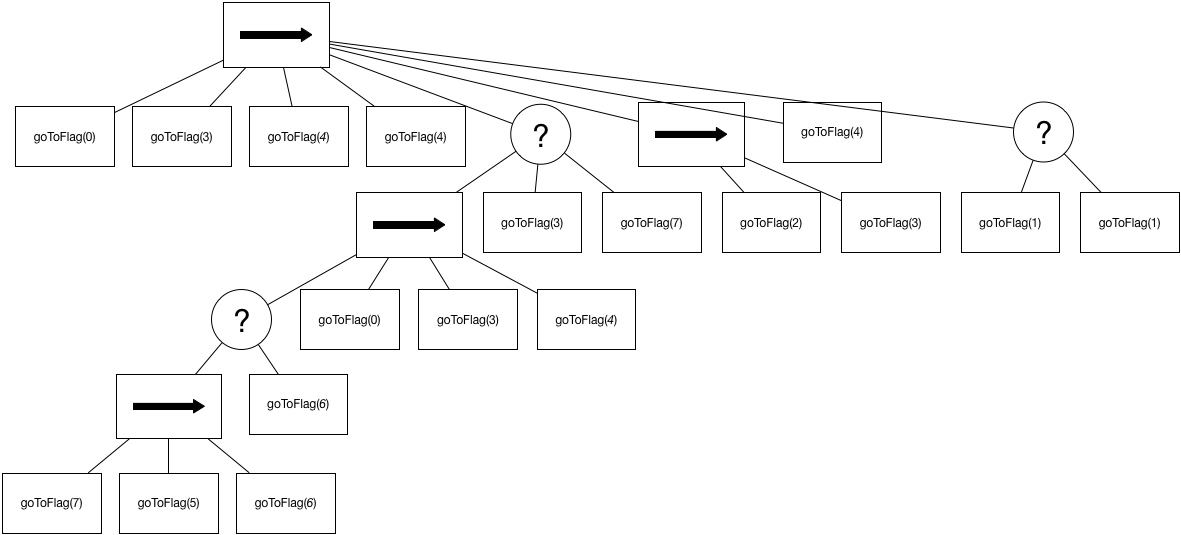
\includegraphics[scale=0.4]{exemplaryspecimenscenario1}
    \caption{Example diagram of a evolutionary generated specimen.}
    \label{fig:x exemplaryspecimenscenario1}
\end{figure}

This particular specimen was generated during one of competitive scenario experimentsand his evaluation placed it on value 5911. Knowing both the value of fitness value constants it can be proven that the specimen claimed 6 resource markers during a simulation lasting 8.7 seconds.

The tree has a very cluttered look and many unnecessary placed nodes, but the route should be clear: going from the top, it's going to visit the closest marker, which is the second one (sic!), then the third, proceeding to the fourth one (twice, in fact, but the second call will return instantly) and head for the last one, only to return to the fifth and sixth, probably meeting a reference agent nearby fifth marker. The rest of the nodes, as mentioned before, serve no function in this particular scenario. Unfortunately, the tree didn't follow the expected strategy (gaining a bit on each marker only to make a final push from sixth to seventh) instead opting to devise a new one. Although - as seen abole - the strategy of choice seems to be at least equally viable.
\section{Optimisation Results}
In this section, results of model cases (one from each scenario) will be presented. When analysing the results, three main components were kept in mind:
\begin{itemize}
    \item The shape of the algorithms' best specimen fitness value and its relation to average fitness value in current iteration.
    \item An average size of a tree in the current population.
    \item A number of iterations needed for the best specimen to achieve success.
\end{itemize}
The shape of fitness plots indicate the general state and health of the Genetic Programming algorithm. While the plot indicating top fitness value in the population is certainly important (the success measure is directly tied to a top specimen, after all), it's the average fitness value in the population that provides the much needed information on population growth, stagnation or even oscillations, indicating local plateaus.

The average size of a tree is also a useful indicator of a general perceived value of the generation: while larger trees are not neccessairly always worse (since the execution time is virtually neglible), they most definietly contain needless constructs. Apart from being nigh unreadable, disregarding tree size would certainly result in need of introducing some kind of post-processing to prune a number of never-to-be-executed branches.

Finally, the number of iterations needed to produce a first solution that is deemed ``successful''. Looking into the matter from the user's perspective,the only feasible characteristic is the speed of achieving a \textit{fit} specimen, able to deal with the task at hand.

Figure \ref{fig:x competitivefitnessplot} presents a plot of the highest fitness value and average fitness in the population in respect to iteration in the competitive scenario. Figure \ref{fig:x competitivetreesizeplot}, hovever, illustrates the change of average tree size in the population in the course of the algorithm's run in the same scenario.

\begin{figure}[h]
    \centering
    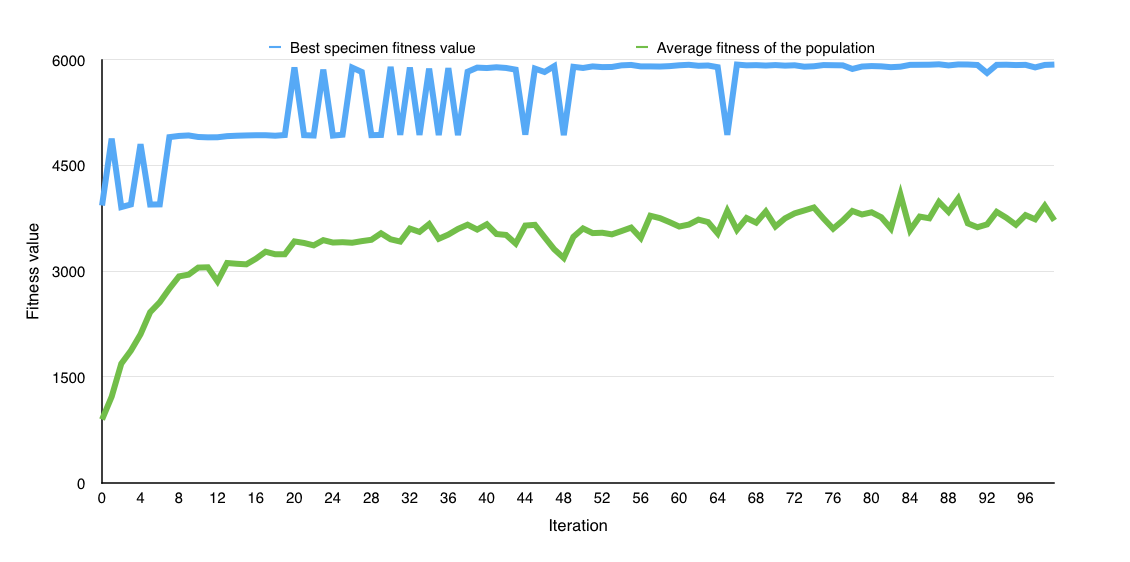
\includegraphics[scale=0.6]{competitivefitnessplot}
    \caption{A fitness value with respect to iteration plot in the competitive scenario.}
    \label{fig:x competitivefitnessplot}
\end{figure}

\begin{figure}[h]
    \centering
    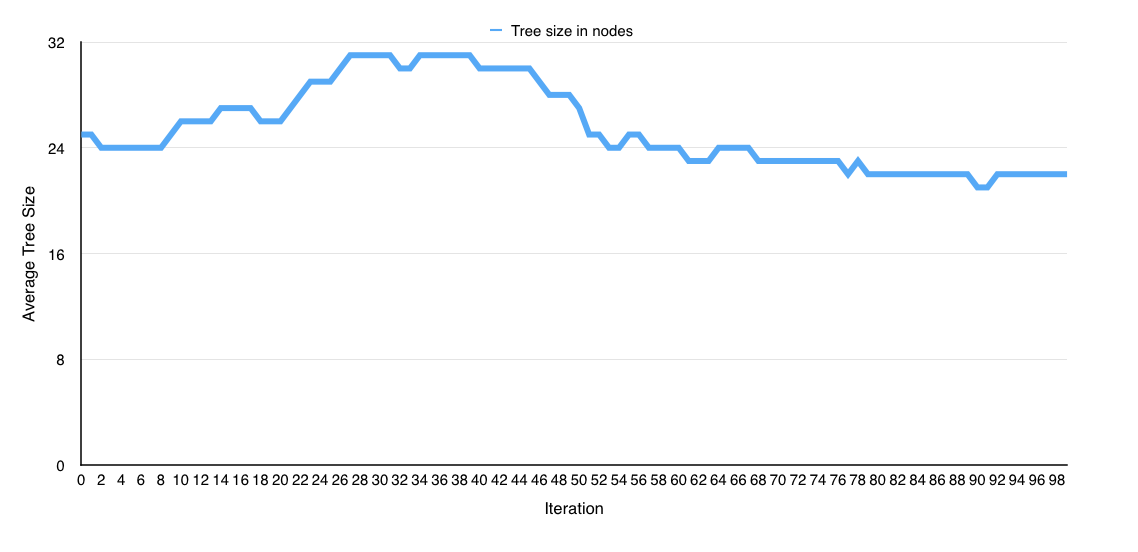
\includegraphics[scale=0.6]{competitivetreesizeplot}
    \caption{An average tree size with respect to iteration plot in the competitive scenario.}
    \label{fig:x competitivetreesizeplot}
\end{figure}
The algorithm's run in this particular case started on a relatively high note, with the best specimen claiming 4 markers for himself. In the next few iterations, best fitness achieved increased, then oscillated around 4200 value, to finally stabilize on a value closer to 5000. Up to this point, one can see the average fitness in the generation rising, indicating that, while there were no radical increases in value, the algorithm is producing more and more feasible options. Then, surely due to particularly good mutation or crossover, a breakthrough is made and the population achieves its first successful specimen. This one, however, is instantly lost, having not been copied over to the next generation. The curve then starts oscillating heavily, with the algorithm producing further successful specimen only to lose them few cycles later. Finally, around iteration 50 mark, the best specimen is kept for a little longer. Note that the first successful individual marked the decline in average fitness growth. That proves that by this time, the population has been saturated with useful gene structures.

The size plot is intended to be considered and analysed together with the previous one. Having done that, one can observe that with the first successful specimen produced, the population started intensively increasing in node count. Having achieved large enough pool of fit solutions, size started to be the diffrentiating factor, successfully lowering the number. This is the perfect example of larger trees being promoted in the initial stages (since they have a larger chance of containing a useful node structure), but having their value decreased as the useful genes from them are passed into further generations. This also poses an interesting question - whether the first found successful specimen should be accepted, or will processing more generations rewarding?

\begin{figure}[h]
    \centering
    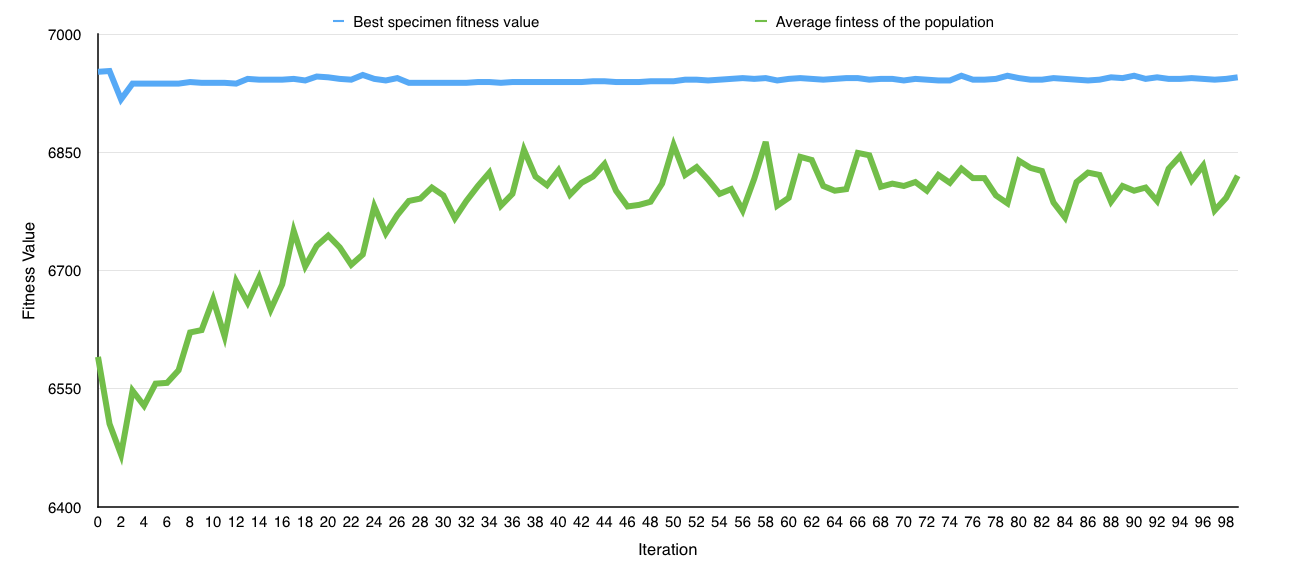
\includegraphics[scale=0.6]{cooperativefitnessplot}
    \caption{A fitness value with respect to iteration plot in the cooperative scenario.}
    \label{fig:x cooperativefitnessplot}
\end{figure}

\begin{figure}[h]
    \centering
    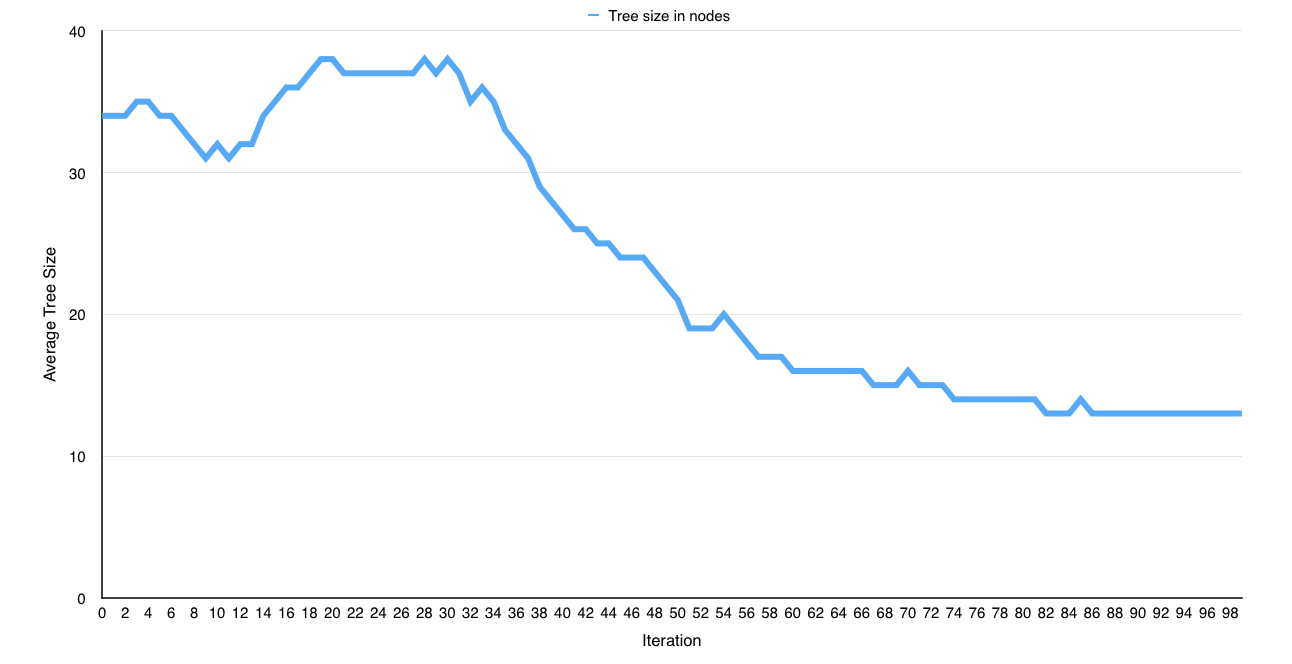
\includegraphics[scale=0.6]{cooperativetreesizeplot}
    \caption{An average tree size with respect to iteration plot in the cooperative scenario.}
    \label{fig:x cooperativetreesizeplot}
\end{figure}

Having seen the competitive scenario, the fitness plot in figure \ref{fig:x cooperativefitnessplot} might not appear as telling at first. Having produced a successful specimen in the first generation, the individual is instantly destroyed, its genes dilluted in the next generation. Another one, however, is produced as quickly as the fourth iteration of the algorithm. The value then remains virtually unchanged, oscillating only slightly to the last generation. Average fitness value curve reflects that progress well, with the oscillations starting only when the other one stabilizes. 

The feeling disappears, however, looking at the average tree size change presented in figure \ref{fig:x cooperativetreesizeplot}. On 30th generation, when the fitness value of the best specimen appears to enter stagnation, abrupt decrease of an average specimen node count begins. Over the next 50 iterations of the algoritm, the average size is reduced almost thrice - from 36 nodes to 13. 
